\section{Results}\label{results}
In this section we describe the results.

%\subsection{Benchmarking}

\begin{figure}[!htbp]
  \centering
    \includegraphics[width=0.9\textwidth]{../figs/gfedComparison.png}
  \caption{Benchmark comparisons against GFED4s \citep{Giglio2013}.}
  \label{fig:benchmark}
\end{figure}

%\subsection{Limitations}

\begin{figure}[!ht]
  \centering
    \includegraphics[width=0.9\textwidth]{../figs/limitation_lines.png}

  \caption{Limitation contribution for each control.}
  \label{fig:lim_lines}
\end{figure}


%\subsection{Sensitivity}

\begin{figure}[!ht]
  \centering
    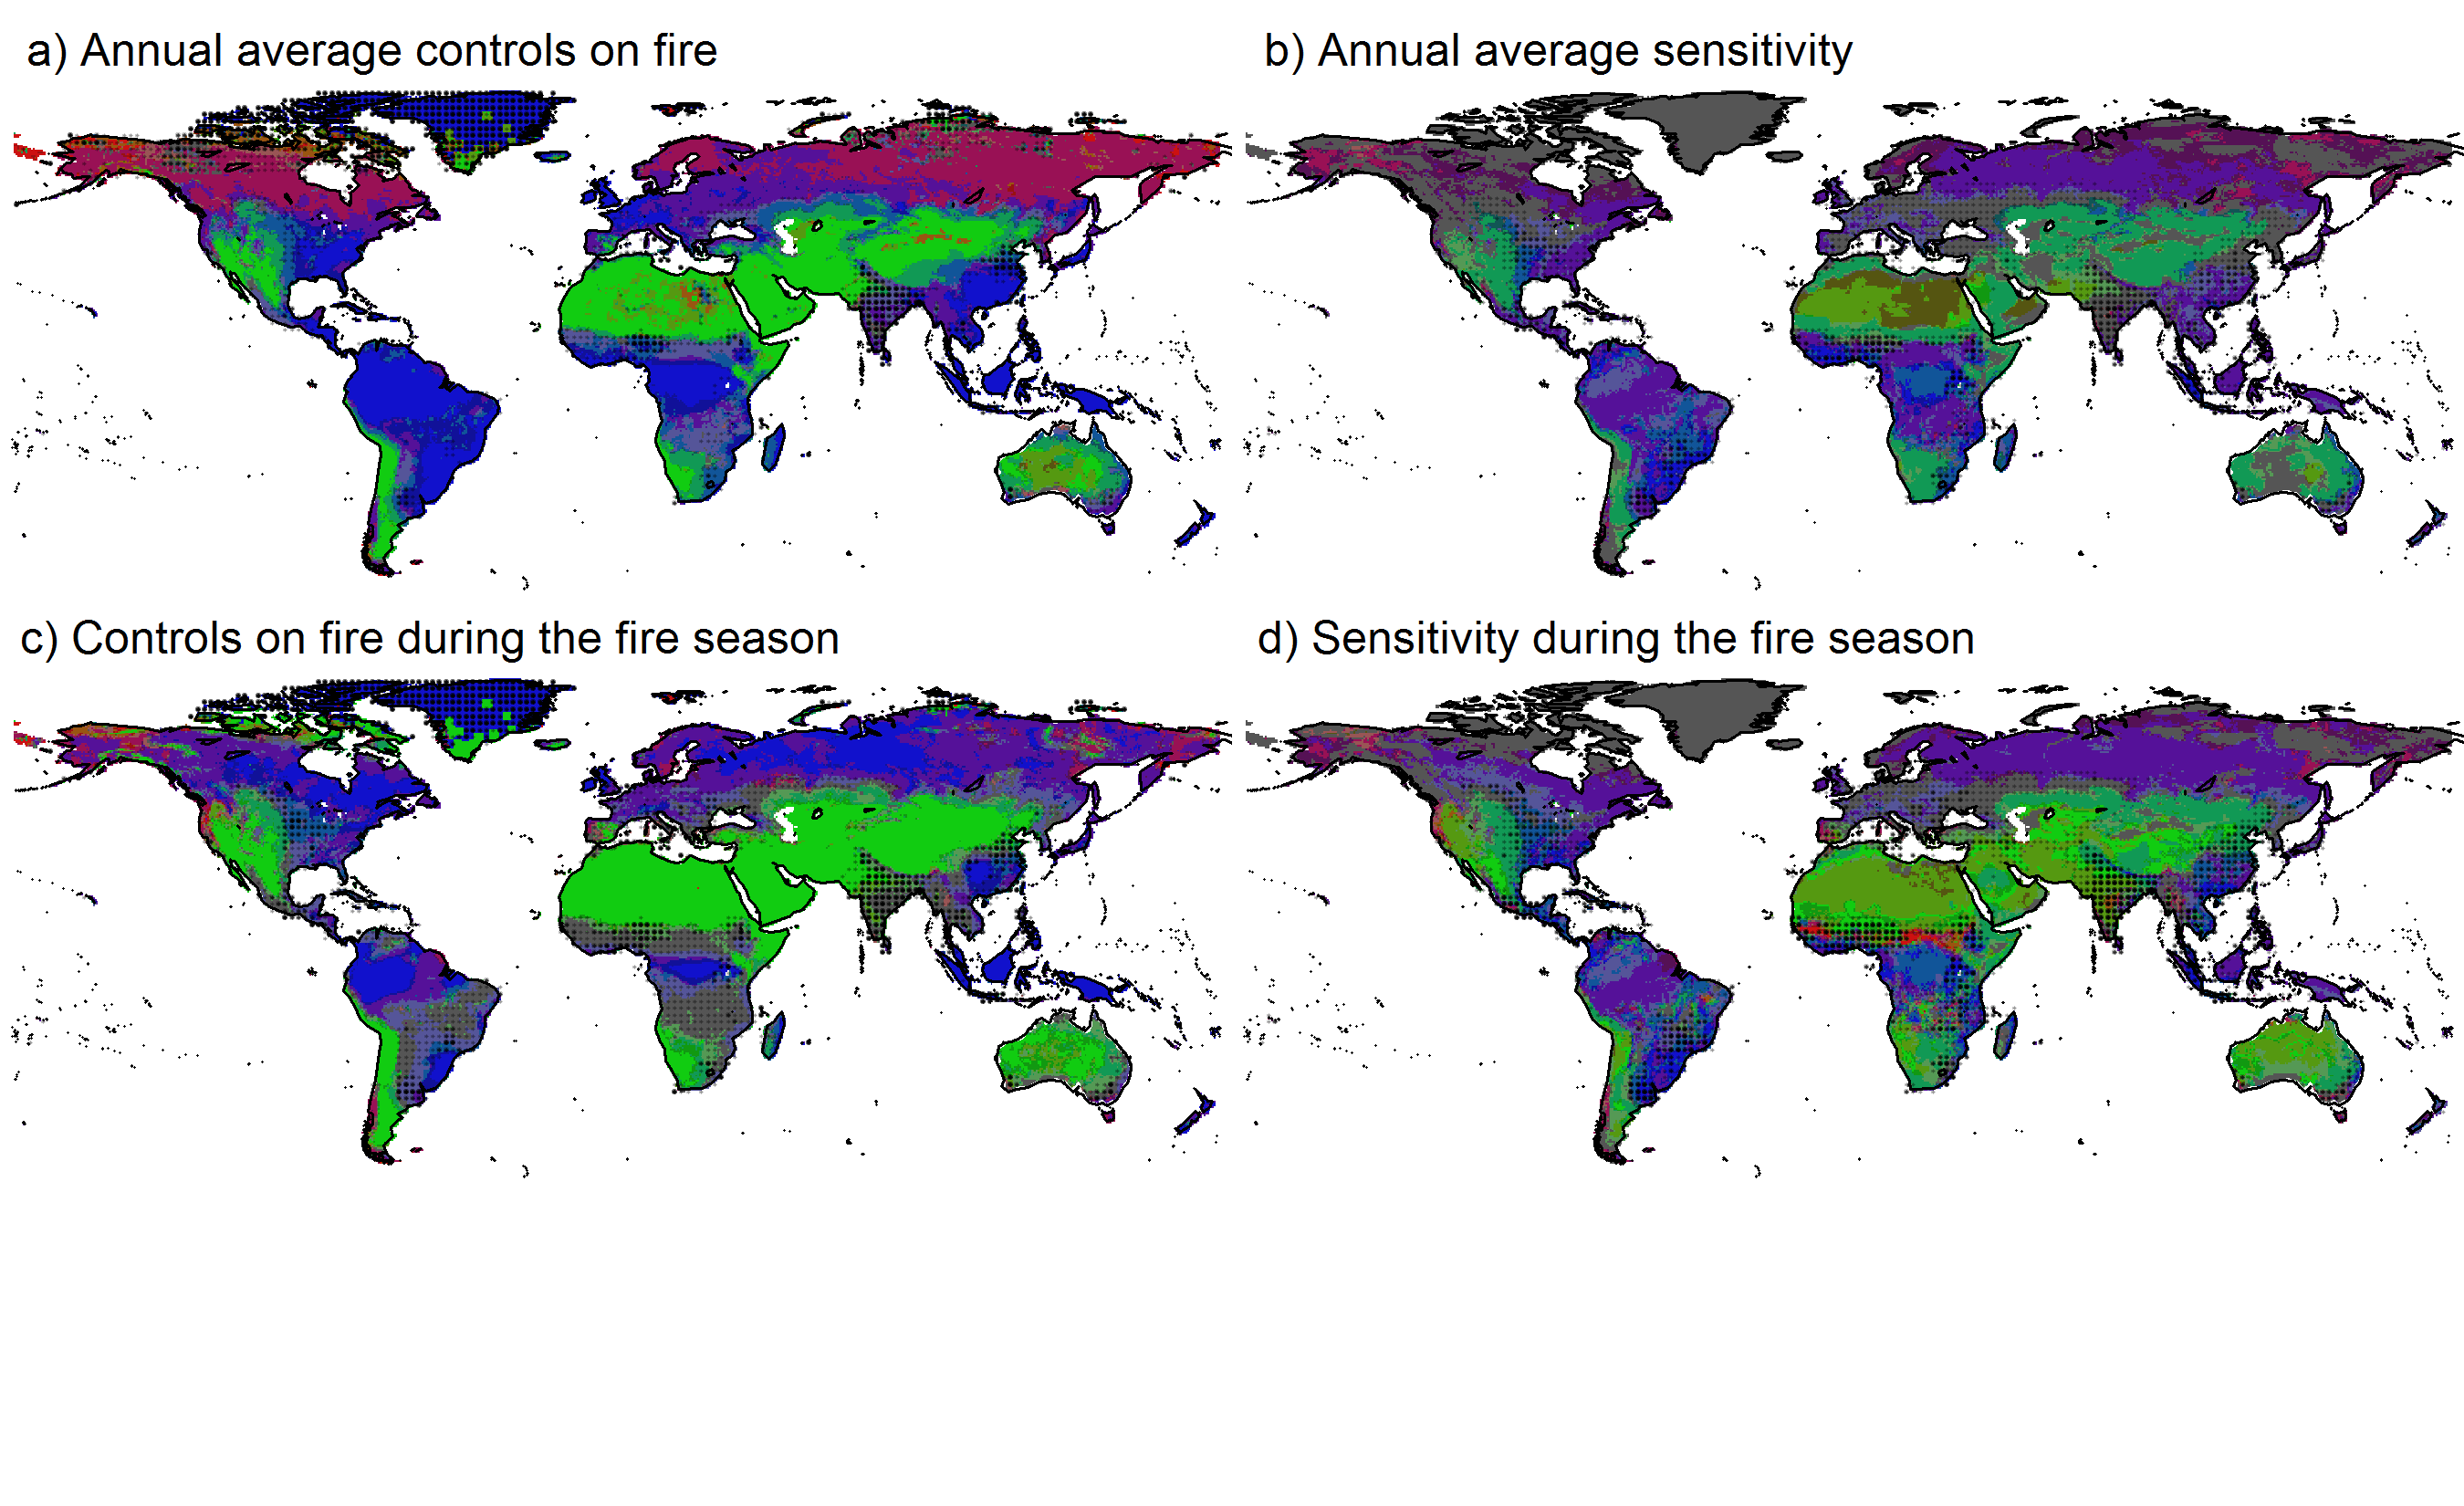
\includegraphics[width=0.9\textwidth]{../figs/limitation_map.png}

  \caption{Limitation and sensitivity.}
  \label{fig:lim_sen_maps}
\end{figure}

\begin{figure}[!ht]
  \centering
    \includegraphics[width=0.67\textwidth]{../figs/moisture_change_for_Amazon_tipping_point.png}

  \caption{Required change in \% fuel moisture content to induce savanna-level fire in the Amazon.}
  \label{fig:amazon}
\end{figure}


%\subsection{Human impact}

\begin{figure}[!ht]
  \centering
    \includegraphics[width=0.9\textwidth]{../figs/HumanImpactMap_small.png}

  \caption{Human impact on burnt area.
            a) Increases in burnt area from human induced fire starts.
            b) Changes in burnt area from human fire starts and suppression.}
    \label{fig:human_impact}
\end{figure}

\begin{figure}[!ht]
  \centering
    \includegraphics[width=0.75\textwidth]{../figs/aguplot_Kelleyetal.png}

  \caption{AGU plot.}
  \label{fig:agu_plot}
\end{figure}


\begin{figure}[!ht]
  \centering
    \includegraphics[width=0.9\textwidth]{../figs/cropland_noCrop_impact.png}

  \caption{The impact of cropland on burnt area in non-cropland within the same grid cell.}
\end{figure}
